\PassOptionsToPackage{full}{textcomp}
\documentclass[%
    a4paper, twoside, dissertation, fontsize=12pt, nobib%
]{tufte-book}
\hypersetup{colorlinks}

%%%%%%%%%%%%%%%%%%%%%%%%%%%%%%%%%%%%%%%%%%%%%%%%%%%%%%%%%%%%%%%%%%%%%%%%%%%%%%%
%% Metadata
\title{data-driven precision cardiology}
\author[Peter Christoffer Holm]{Peter Christoffer Holm}
\publisher{University of Copenhagen}

%%%%%%%%%%%%%%%%%%%%%%%%%%%%%%%%%%%%%%%%%%%%%%%%%%%%%%%%%%%%%%%%%%%%%%%%%%%%%%%

\usepackage[%
    style=verbose-note,
    %style=verbose-note,
    url=false,
    isbn=false,
    doi=false,
    maxcitenames=2,
    sorting=none,
    autocite=footnote,
]{biblatex}
\addbibresource{assets/pch-thesis.bib}

\AtEveryCitekey{\clearfield{pagetotal}}
\AtEveryCitekey{\clearfield{pages}}
\AtEveryCitekey{\clearfield{eprint}}

%%%%%%%%%%%%%%%%%%%%%%%%%%%%%%%%%%%%%%%%%%%%%%%%%%%%%%%%%%%%%%%%%%%%%%%%%%%%%%%

\usepackage[p, osf]{ETbb} % osf in text, tabular lining figures in math
\usepackage[scaled=.95,type1]{cabin} % sans serif in style of Gill Sans

% \usepackage[varqu,varl]{zi4} % inconsolata typewriter

\usepackage{microtype}
\usepackage{booktabs}
\usepackage{lipsum}
\usepackage{pdfpages}
\usepackage{blindtext}
\usepackage{appendix}
\usepackage{amsmath}

% quotation marks
\usepackage{csquotes}

% For graphics / images
\usepackage{graphicx}
\setkeys{Gin}{width=\linewidth,totalheight=\textheight,keepaspectratio}
\graphicspath{{graphics/}}

% The fancyvrb package lets us customize the formatting of verbatim
% environments.  We use a slightly smaller font.
\usepackage{fancyvrb}
\fvset{fontsize=\normalsize}

% Hanging parentheses and asterisks
\newcommand{\hangp}[1]{\makebox[0pt][r]{(}#1\makebox[0pt][l]{)}}
\newcommand{\hangstar}{\makebox[0pt][l]{*}}

% Prints the month name (e.g., January) and the year (e.g., 2008)
\newcommand{\monthyear}{%
  \ifcase\month\or January\or February\or March\or April\or May\or June\or
  July\or August\or September\or October\or November\or
  December\fi\space\number\year
}

% Custom macros
\newcommand{\na}{\quad--}
\newcommand{\blankpage}{\newpage\hbox{}\thispagestyle{empty}\newpage}

%%%%%%%%%%%%%%%%%%%%%%%%%%%%%%%%%%%%%%%%%%%%%%%%%%%%%%%%%%%%%%%%%%%%%%%%%%%%%%%

\begin{document}
\frontmatter
\maketitle

\begin{@empty}
~\vfill
\thispagestyle{empty}
\setlength{\parindent}{0pt}
\setlength{\parskip}{\baselineskip}

\smallcaps{Candidate}

\textbf{Peter Christoffer Holm}, MSc

Novo Nordisk Foundation Center for Protein Research,
University of Copenhagen, Denmark

\smallcaps{Supervisors}

\textbf{Søren Brunak}, PhD, Professor 
(principal supervisor)

Novo Nordisk Foundation Center for Protein Research, 
University of Copenhagen, Denmark

\textbf{Henning Bundgaard}, PhD, Dr.Med, Professor 
(co-supervisor)

Department of Cardiology,
Copenhagen University Hospital, Denmark

\textbf{Karina Banasik}, PhD, Associate Professor 
(co-supervisor)

Novo Nordisk Foundation Center for Protein Research, 
University of Copenhagen, Denmark

\vspace{2em}

\par\smallcaps{Published by the \thanklesspublisher}

\vspace{5em}

\par This document was created using the \LaTeX{} typesetting software.
The layout is based on the \texttt{tufte-latex} document class,
and the main body of the text is set in \textsf{ETbb} and \textsf{Libertine}.
Unless otherwise indicated, all figures and graphics in the main text
are either the property of the author or are in the public domain.

%\par\textit{First printed, \monthyear}

Copyright \copyright\ \the\year\ \thanklessauthor
\end{@empty}

\begin{@empty}
\thispagestyle{empty}
\setlength{\parindent}{0pt}
\setlength{\parskip}{\baselineskip}

\chapter*{Preface}

This PhD thesis has been submitted
to the Graduate School of Health and Medical Sciences,
University of Copenhagen.

The work presented in this thesis was performed
at the Novo Nordisk Foundation Center for Protein Research (CPR),
University of Copenhagen, Denmark.

I declare no conflicts of interests.

\begin{flushright}
    Copenhagen, December 2023 \\
    Peter Christoffer Holm
\end{flushright}
\end{@empty}


\cleardoublepage
 
\tableofcontents
\listoffigures
\listoftables
\cleardoublepage

%%%%%%%%%%%%%%%%%%%%%%%%%%%%%%%%%%%%%%%%%%%%%%%%%%%%%%%%%%%%%%%%%%%%%%%%%%%%%%%

\mainmatter

\chapter{Summary}
\chapter{Scientific Publications}

%%%%%%%%%%%%%%%%%%%%%%%%%%%%%%%%%%%%%%%%%%%%%%%%%%%%%%%%%%%%%%%%%%%%%%%%%%%%%%%

\part{General Introduction}

\chapter{Data-driven Precision Medicine} \label{precision-medicine}

A 2013 Cochrane review on \citetitle{taylorStatins2013} concluded 
that statins effectively lower all-cause mortality and reduce the incidence
of both fatal and non-fatal cardiovascular events all without any serious
adverse effects~\autocite{taylorStatins2013}.
For instance, the relative risk of fatal cardiovascular events 
when using statins as opposed to placebo
was estimated to \num{0.82} with a 
\si{95}{\%} \ac{CI} of \num{0.70} to \num{0.96}.
~\autocite{taylorStatins2013}
This means that those treated with statins, on average,
are \si{18}{\%} less likely to die from cardiovascular causes. 
However, it is important to emphasize that this \si{18}{\%} 
reduction is an average effect.
There might be groups of people for whom the reduction could be 
even higher, while others may see little to no benefit. 
Understanding and making use of such individual variability 
is the central objective of precision medicine.

As a concept, precision medicine is not a new idea;
tissue- and blood typing, for instance,  
has been used to guide treatment for many decades.
However, the prospective of leveraging large clinical databases
and broad array of phenotypic information 
to deliver precision medicine across
a wide spectrum of disease states
is adding renewed interest in the concept.






Use data to improve decision making


Subgroup identification seeks to identify groups of individuals with an
increased treatment response, which
\citeauthor{kosorokPrecision2019} refers to as 
\textquote[kosorokPrecision2019]{%
    finding the right patient for the right treatment%
}.


\begin{table*}[h]
    \footnotesize
    \centering
    \begin{tabularx}{0.9\textwidth}{XlX} \toprule
    Condition & Gene & Action \\
    \midrule
    Familial hypercholesterolaemia & \textit{PCSK9}, \textit{APOB}, and \textit{LDLR} & Indication for PCSK9 inhibitor drugs \\
    Familial hypercholesterolaemia & \textit{PCSK9}, \textit{APOB}, and \textit{LDLR} & Indication for PCSK9 inhibitor drugs \\
    Familial hypercholesterolaemia & \textit{PCSK9}, \textit{APOB}, and \textit{LDLR} & Indication for PCSK9 inhibitor drugs \\
    Familial hypercholesterolaemia & \textit{PCSK9}, \textit{APOB}, and \textit{LDLR} & Indication for PCSK9 inhibitor drugs \\
    Chronic myeloid leukemia       & BCR/ABL & Imatinib \\
    Chronic myeloid leukemia       & BCR/ABL & Imatinib \\
    Chronic myeloid leukemia       & BCR/ABL & Imatinib \\
    Chronic myeloid leukemia       & BCR/ABL & Imatinib \\
    Chronic myeloid leukemia       & BCR/ABL & Imatinib \\
    \bottomrule
    \end{tabularx}
    \caption[Precision drugs]{
        Examples of precision pharmacotherapy informed by genetics 
        and more more more more
    }
\end{table*}



Electronical health records are a rich source of health data,
and can be used to find connections between risk factors and diseases.

Precision medicine is prevention and treatment approaches
that takes individual variation into account.


The terms
\enquote{precision},
\enquote{personalized},
and \enquote{individualized medicine}
are often used interchangeably.






\section{Deep phenotyping} \label{deep-pheno}

In their review 
\citetitle{konigWhat2017}, 
\citeauthor{konigWhat2017} presents data-driven precision medicine
as a framework with three main \enquote{tracks} or \enquote{processes}
that serves as an useful abstraction for understanding
the process of moving from big data
to clinically actionable insights~%
\autocite{konigWhat2017}. 
At the center of the framwork resides the data,
which are both plentiful and representative of the population of interest.
Now, the three tracks are
1) preprocessing and data-mining
2) diagnostic and prognostic models
and 3) prediction of treatment response.

\subsection{Track 1: preprocessing and data mining}

Quality control, preprocessing, and extraction of information.
The concrete steps and methods utilized as part of this track
is highly context-dependent, 
and is therefore difficult to describe on a general level. 

Feature-engineering.

Extracting structured information from unstructured information.

Clustering.

\subsection{Track 2: diagnostic and prognostic models}

Relying in part on processed data from track 1
as well as any insights gained from data-mining,
track 2 is concerned with the development
of models that can characterise current (diagnostic models)
or future (prognostic models) states of health and disease~%
\autocite{konigWhat2017}. 

\subsection{Track 3: predicting treatment response}

\todo[inline, caption={Some text}]{
\begin{minipage}{\linewidth}
    \emph{Notes:}

    Causality.
    Different strategies exists for guiding the development of 
    predicting therapy response.
    We might be able to use prognostic and diagnostic factors
    discovered in the previous track to predict treatment response.
    Example: HER is prognostic for survival in breast cancer,
        but is also predictive of treatment response against X.


\end{minipage}
}

As with the other tracks, track 3 gan generate further knowledge 
that in turn can feed back to the more general phenotyping of patients
\autocite{konigWhat2017}. 


\section{Health Informatics}

Health informatics is a cross-disciplinary field
that aims at developing methods and techniques
for the collection, study, and analysis of healthcare data.
It operates in the intersection between medicine and computer science,
and involves disciplines such as
bioinformatics, software engineering, statistics, information systems,
data science, and artificial intelligence.
The overall goal of health informatics is the data-driven improvement
of delivery and accuracy of health and healthcare for the individual patient.

In modern medicine, 
ever increasing amounts of data 
is continuously being generated and collected.
Ranging from structured administrative data 
used primarily for billing purposes
to advanced imaging and high-througput \enquote{omics} analyses,
the array of available data is as diverse as it is plentiful.

The volume and range of information collected
at just a single visit for a single patient
can be large.


There is increasing evidence that informatics improves
health care, public health, and biomedical research.

    
An electronic health record
is a systematized collection of health data 
stored in a digital format.
Electronic health records may include data such as
medical history, drug prescriptions, laboratory test results,
radiology images, body measurements, and billing information.
EHRs enable following patients in both time and space;
not only in the physical space that is the cardiology department
and the intensive care unit, but also in the health-and-disease space.

\begin{itemize}
    \item \textbf{Decision support systems}
    \item \textbf{Personalized medicine}
    \item \textbf{Mobile health applications} (aka. \textit{mHealth})
    \item \textbf{Screening}
    \item \textbf{Surveillance}
    \item \textbf{Medical outcomes}
\end{itemize}

\marginnote{
    The five Vs of big data:
    \begin{itemize}
        \item Volume
        \item Velocity
        \item Variety
        \item Value
        \item Veracity
    \end{itemize}
}

\section{Clinical decision support systems}

Deep learning can identify patterns in sparse, noisy,
and very heterogenous data without the need for expert feature engineering
\cite{norgeotCall2019}.

Challenges in developing machine learning models from electronic health records
includes syntactic interoperability, 
which specifies the format and structure of the data.
Many different interopability formats exists, 
but their adoption varies considerably.

Benefits of interopable digital health data
~\autocite{lehneWhy2019}.
Test~\cite{lehneWhy2019}.

\begin{itemize}
    \item Large-scale observational studies.
    \item Less time spend on data cleaning and pre-processing.
    \item Interoperable exchange format could further cross-institutional
    and international collaboration, which would make it easier 
    to reproduce and externally validate e.g. prognostic applications.
    In the case of rare diseases with very limited number of patients, 
    international pooling of data could enable analysis
    that otherwise would not be possible.
    \item Faster research and development process.
    \item If data is known to conform to a well-defined format,
    computer software can be written without explicit access to the data.
    This solve many issues related to sensitive data or
    data that are otherwise subject to strict data protection regulations.
\end{itemize}


Healthcare data are usually private and scattered across various applications,
which makes it difficult to share data and generate robust results 
that translate to different and diverse populations.


Succesful implementation of data-driven applications
require large and diverse data sets.

AI approaches rely on data that accurately represent
the real-life distribution of the underlying problem.
We can not exclusively rely on data that have been carefully curated 
from few and often very similar sources. 
In order to capture subtle relationships 
between health and disease patterns,
we need to include many and diverse cases~%
\autocite{riekeFuture2020}.

Federated learning could solve some of these issues\autocite{riekeFuture2020}.





\chapter{Health Informatics}

Health informatics is a cross-disciplinary field
that aims at developing methods and techniques
for the study of healthcare data.

It operates in the intersection between medicine and computer science,
and involves disciplines such as
bioinformatics, software engineering, statistics, information systems,
data science, and artificial intelligence.

The goal of health informatics is the data-driven improvement
of delivery and accuracy of healthcare to the individual patient.
    
An electronic health record
is a systematized collection of health data 
stored in a digital format.
Electronic health records may include data such as
medical history, drug prescriptions, laboratory test results,
radiology images, body measurements, and billing information.
EHRs enable following patients in both time and space;
not only in the physical space that is the cardiology department
and the intensive care unit, but also in the health-and-disease space.

\begin{itemize}
    \item \textbf{Decision support systems}
    \item \textbf{Personalized medicine}
    \item \textbf{Mobile health applications} (aka. \textit{mHealth})
    \item \textbf{Screening}
    \item \textbf{Surveillance}
    \item \textbf{Medical outcomes}
\end{itemize}

\marginnote{
    The five Vs of big data:
    \begin{itemize}
        \item Volume
        \item Velocity
        \item Variety
        \item Value
        \item Veracity
    \end{itemize}
}

\section{Clinical decision support systems}

Deep learning can identify patterns in sparse, noisy,
and very heterogenous data without the need for expert feature engineering
\cite{norgeotCall2019}.




\chapter{Machine Learning}

The promise of AI lies in the ability 
to integrate large amounts of data from huge data sets
and almost instantaneously register patterns
with clinical importance.

Machine Learning seeks to let computers learn from data
without them being explicitly programmed.


The Turing test, proposed by Alan Turing in 1950,
tries to answer the question \enquote{can a machine think?}.
A computer passes the test if a human interogator,
after posing a series of written questions,
cannot determine if the responses come from a human or a computer.


\textquote[\autocite{russellArtificial2009}]{%
The quest for \enquote{artificial flight} succeeded 
when engineers and inventors stopped imitating birds 
and started using wind tunnels and learning about aerodynamics.
Aeronautical engineering texts 
do not define the goal of their field as making 
\enquote{machines that fly so exactly like pigeons 
that they can fool other pigeons.}\,}

If the output is a finite set of values
the learning problem is called \textbf{classification},
and if it is a number, then it is called \textbf{regresion}.

In supervised learning, the model observes input-output pairs
and tries to learn a function that maps inputs to outputs.

In unsupervised learning, the model learns patterns in unlabeled input data.

With many machine-learning models, there is a bias--variance tradeoff:
on one end of the spectrum we have simple low-variance models 
such as linear or logistic regression
and on the other end, we have high-variance models
such as neural networks or random forests.

We can estimate the error rate of model
by evaluating it on a test set.
If we are only creating a single model,
then this approach suffices. 
However, we might want to compare many different models,
or slightly tweak an already existing model,
such that we can select the performing version.
If we select the final model based on the test set,
we might inadvertently have biased the process,
and could, in a sense, have overfitted to the test data.
To avoid this, we need to completely hide away the test data
until we are done with training, experimenting, 
and hyperparameter optimization.
To allow this, we instead need three sets of data:

\begin{itemize}
    \item a training set to train or develop candidate models
    \item a validation set to evaluate the candidate models
        and select the best one
    \item a test set do the final unbiased evaluation of model performance
\end{itemize}

Another alternative is using the technique \textit{k}-fold cross-validation.

A model is interpretable if we can inspect the model
and understand why it gave a certain output for a particular input.
An explainable model is one that can help us understand 
why a certain output was produced for a specific input.
Interpretability comes from inspecting the actual model.
Explainability can come from an external process.

Typically there is a distinction between model-based explanations
and post hoc explanations\autocite{vanderveldenExplainable2022}.
The scope of an explanation is the difference between
explanations for a complete model and
explanations for a single output.
Global explanation covers feature importance estimates 
for the entire dataset.
Local explanations, on the other hand, seeks to explain
the impact of the specific example under scrutiny.
A SHAP-waterfall plot is an example of a local explanation.
A saliency map of a chest radiograph that shows
which pixels contributed to the label \enquote{liver cancer}
is another example.

Shapley values measures the marginal contribution
of each individual feature.

One limitation of XAI models is the accuracy and relevance of explanations.
Explainability algorithms such as SHAP are only approximations
of the complete model.
In other words, the fidelity is not perfect and therefore neither
is the explanation.
However, for black-box models such as neural networks,
it is the next best thing.

\section{Neural Networks}

\begin{marginfigure}%
	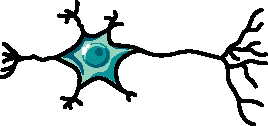
\includegraphics[width=\linewidth]{graphics/neuron}
    \caption[Schematic diagram of a neuron]{%
        Schematic diagram of a neuron.
        A typical neuron has a dendrites, a cell body, and a single axon; 
        the dendrites receive input signals from other neurons,
        and propagates output signals along the axon.
    }
    \label{fig:neuron}
\end{marginfigure}

\begin{marginfigure}%
	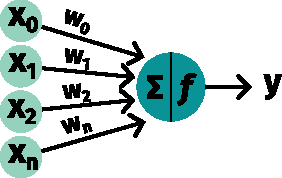
\includegraphics[width=\linewidth]{graphics/perceptron}
	\caption{Schematic diagram of a perceptron}
    \label{fig:perceptron}
\end{marginfigure}

%%%%%%%%%%%%%%%%%%%%%%%%%%%%%%%%%%%%%%%%%%%%%%%%%%%%%%%%%%%%%%%%%%%%%%%%%%%%%%%

Neural networks have been designed
using the archicteture of neurons in a human brain as inspiration.
The simplest model is that of a perceptron, 
which can be seen as a computational approximation
of a real neuron or nerve cell%
\autocite{charniakIntroduction2019}.
A typical neuron has many dendrites, a cell body, and a single axon 
(Figure~\ref{fig:neuron}).
The dendrites carries the input signal to a neuron,
and if the cumulative signal is great enough%
\sidenote{
    This threshold is known as 
    the \textit{threshold potential},
    and is typically between -50 and -55 mV.
}, 
then the neuron will propagate an action potential down the axon%
\autocite{seifterConcepts2005}.
In similar fashion, a perceptron receives may receive many different inputs
and produces a single output (Figure~\ref{fig:perceptron}).
In the case of a neuron, the \enquote{all-or-none} principle means
that nerve cells either signals at full strength or not all.
For a perceptron, this priniciple can be emulated
with the followingly step function:

\begin{equation}
    f_{\phi}(\mathbf{x})  = 
        \begin{cases}
            1 & \text{if } b + \mathbf{w} \cdot \mathbf{x} > 0\\
            0 & \text{otherwise}
        \end{cases}
\end{equation}

By combing many thousands of such neurons,
in a multilayer-perceptron or artificial neural network,
we can create a model that, 
can learn even the most complex of patterns.
Deep learning is at its core a form of representation learning.
Each layer in a neural network is a different representation,
and by stacking several of such layers on top of each others,
the representation in one hidden layer
feeds into the next layer and
is thereby being transformed into an even more abstract representation%
\autocite{estevaGuide2019}.

%%%%%%%%%%%%%%%%%%%%%%%%%%%%%%%%%%%%%%%%%%%%%%%%%%%%%%%%%%%%%%%%%%%%%%%%%%%%%%%
% insert example of abstract representations in a computervis model
%%%%%%%%%%%%%%%%%%%%%%%%%%%%%%%%%%%%%%%%%%%%%%%%%%%%%%%%%%%%%%%%%%%%%%%%%%%%%%%


\section{Regularization}

One approach to avoid overfitting in neural networks
is a technique known as dropout.
At each step of model training,
a random set of nodes in the network are disabled.
In a sense, the result is a rough approximation of 
an ensemble of different networks.


Dropout introduces noise during training
and thereby forces the network to be less senstive of noise.
Hidden units trained with dropout needs to be useful 
with or without the presence of neighboring units.

%%%%%%%%%%%%%%%%%%%%%%%%%%%%%%%%%%%%%%%%%%%%%%%%%%%%%%%%%%%%%%%%%%%%%%%%%%%%%%%

\section{Miscellaneous}

In his review on artificial intelligence in medicine%
\autocite{topolHighperformance2019}, 
Eric Topol expresses his view that in the future
\blockquote{%
almost every type of clinician, ranging from specialty doctor to paramedic,
will be using AI technology, and in particular deep learning [...]
}.

The ability to predict adverse outcomes could make  
healthcare resources more efficient.

Systematic deugging and continuous monitoring and validation 
is of utmost importance if we are to release AI algorithms into the wild%
\autocite{topolHighperformance2019}.

There has been much discussion about, and there are many opinions on, 
the black-box nature of many machine learning algorithms and 
how it should or should not affect the clinical use of such 
\autocite{topolHighperformance2019, gunningXAI2019, vanderveldenExplainable2022}.


In computer vision tasks in the medical domain,
deep-learning models have achieved physician-level performance
in many different diagnostic tasks
ranging from \todo{finish sentence}.


%%%%%%%%%%%%%%%%%%%%%%%%%%%%%%%%%%%%%%%%%%%%%%%%%%%%%%%%%%%%%%%%%%%%%%%%%%%%%%%

\backmatter

\printbibliography

%%%%%%%%%%%%%%%%%%%%%%%%%%%%%%%%%%%%%%%%%%%%%%%%%%%%%%%%%%%%%%%%%%%%%%%%%%%%%%%

\part*{Appendix}

\appendix

\chapter{Paper 1}
\chapter{Paper 1}

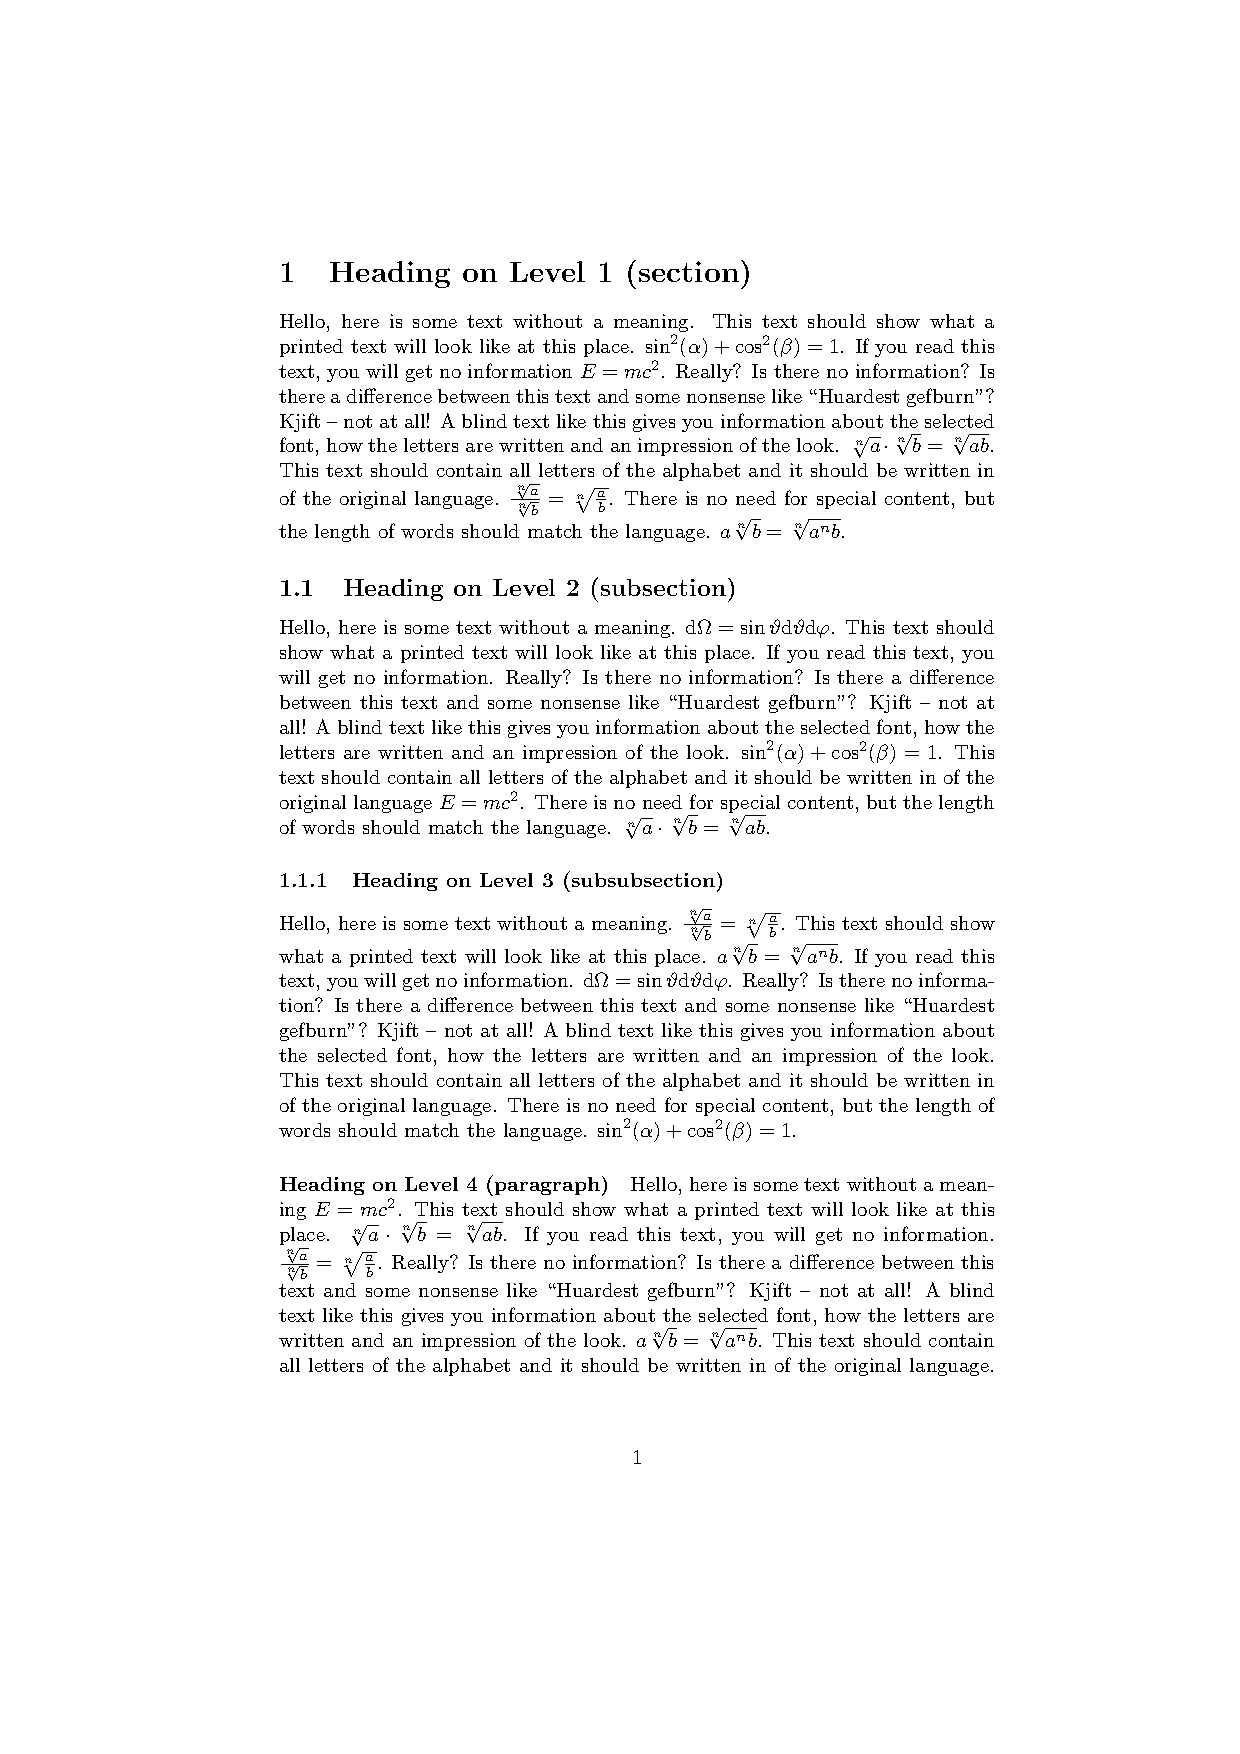
\includepdf[%
    frame=true, scale=0.8, pages=-, pagecommand={}%
]{assets/dummy.pdf}

\end{document}
